% 第三部分 C 结果：树状 GRPO 训练（由 main_zh.tex 引入）。

\section{用树状 rollout 训练}\label{sec:res-tree}

两种树状条件各用 \NUM{seeds_treekev} 个种子训练 200 步，其余一切与第二部分的 \texttt{rlvr} 相同；\texttt{rlvr} 是扁平采样的参照（\NUM{seeds_rlvr} 个种子）。种子相同的 run 以相同的顺序看到相同的题目。我们先为每种树状条件跑了两个种子。那时每种条件都有一个种子远高于 \texttt{rlvr}、另一个与它持平，树形的作用无法判断，于是在两个种子都跑完之后，我们为每种条件各加了第三个种子（\file{scripts/make_jobs.sh}）。这一决定是在看到前两个种子的结果之后做出的；第三个种子与其他种子一样报告。表~\ref{tab:tree-acc} 给出最终准确率，表~\ref{tab:tree-seeds} 给出每个种子的准确率，表~\ref{tab:tree-paired} 给出配对差，表~\ref{tab:tree-stats} 给出训练期间树内部的情况，图~\ref{fig:tree-curves} 给出训练曲线。区间按题目重采样，不包含种子之间的差异。

\subsection{评判模型的选根}\label{sec:res-tree-choice}

\paragraph{评判模型的选择比随机选择好不了多少。} 每隔十步，未被保留的根也会被续写，因此我们知道保留所选的两个根相对于保留全部四个根带来了多少收益（表~\ref{tab:tree-stats}）。在 \texttt{tree\_kev} 下，\kev{} 排得最高的两个根的叶子，比全部四个根的叶子正确的频率高 \NUM{auditgain_all_treekev} \ci{\NUM{auditgainlo_all_treekev}}{\NUM{auditgainhi_all_treekev}} 个百分点（共 \NUM{auditgain_records_treekev} 个审计步）。在 \texttt{tree\_random} 下，选择在期望上没有任何收益，同一个数为 \NUM{auditgain_all_treerand} \ci{\NUM{auditgainlo_all_treerand}}{\NUM{auditgainhi_all_treerand}}；这些区间对审计步重采样。保留事后叶子表现最好的两个根，可以获得 \NUM{auditbest_all_treekev} 个百分点的收益；这比任何在叶子出现之前做出的排序所能达到的都多，因为每个根的同样四个叶子既用于给根排序，又用于计分。在审计步上，\kev{} 对一个根的 \emph{on track} 分数区分该根正确与错误叶子的 AUROC，合并所有提示时为 \NUM{auditotauc_all_treekev}，在提示内部却只有 \NUM{auditotaucw_all_treekev} \ci{\NUM{auditotaucwlo_all_treekev}}{\NUM{auditotaucwhi_all_treekev}}，而决定保留哪些根的正是提示内部的比较（\texttt{tree\_random} 下为 \NUM{auditotaucw_all_treerand}）。离线时在相同的结构下（每题四个 128 词元的前缀，每个前缀续写四次），题目内部的 AUROC 为 \NUM{aucw_128_kevtrack}，保留排得最高的两个前缀让最终正确的续写比例提高了 \NUM{gainpt_128_kevtrack} 个百分点（\S\ref{sec:res-prefix}）。两者的前缀不同：离线时是基座策略的前缀，训练中是策略在学习过程中自己的前缀。它的根越来越常导向正确答案（在 \texttt{tree\_random} 下，训练前半段被审计的叶子中有 \NUM{auditval_firsthalf_treerand}\% 正确，后半段为 \NUM{auditval_secondhalf_treerand}\%；离线时基座策略前缀的续写中为 \NUM{ps_valueallpct_128}\%），选择的余地——事后最好的两个根——也从 \NUM{auditbest_firsthalf_treerand} 个百分点缩小到 \NUM{auditbest_secondhalf_treerand} 个百分点。

\begin{table}[t]
\centering\small\setlength{\tabcolsep}{5pt}
\begin{tabular}{@{}lcccccccc@{}}
\toprule
 & & roots & \multicolumn{5}{c}{audit, every 10th step: all four roots continued} & tokens \\ \cmidrule(lr){4-8}
condition & seeds & ended & AUROC & within prompt & value & gain, kept 2 & gain, best 2 & per step (k) \\ \midrule
\texttt{tree\_random} & 3 & 1.5\% & 0.75 & 0.56 & 60.6 & $+$0.3 & $+$8.1 & 65.1 \\
\texttt{tree\_kev} & 3 & 1.3\% & 0.75 & 0.55 & 59.9 & $+$1.4 & $+$8.4 & 74.7 \\
\bottomrule
\end{tabular}

\caption{训练期间树的内部情况（对步数和种子取平均）：在 128 个词元内已经结束的根的比例；在审计步上（每十步一次，一个提示的四个根都被续写），\kev{} 对根的 \emph{on track} 分数对其叶子验证结果的 AUROC（合并与提示内部）、全部四个根的叶子准确率（\%），以及保留所选的两个根或事后最好的两个根相对于它的收益（百分点）；每步生成的词元数（千，最后 20 步），不含审计的续写。}
\label{tab:tree-stats}
\end{table}

\paragraph{最终准确率：评判模型的选择没有作用。} 在相同的树形下，用 \kev{} 选的根代替随机选的根，最终准确率的变化在 MATH-500 上为 \NUM{dvtreerand_treekev_math} \ci{\NUM{dvtreerandlo_treekev_math}}{\NUM{dvtreerandhi_treekev_math}} 个百分点，在 GSM8K 上为 \NUM{dvtreerand_treekev_gsm} \ci{\NUM{dvtreerandlo_treekev_gsm}}{\NUM{dvtreerandhi_treekev_gsm}}，在 AMC23 上为 \NUM{dvtreerand_treekev_amc} \ci{\NUM{dvtreerandlo_treekev_amc}}{\NUM{dvtreerandhi_treekev_amc}}，在 AIME24 上为 \NUM{dvtreerand_treekev_aime24} \ci{\NUM{dvtreerandlo_treekev_aime24}}{\NUM{dvtreerandhi_treekev_aime24}}，在 AIME25 上为 \NUM{dvtreerand_treekev_aime25} \ci{\NUM{dvtreerandlo_treekev_aime25}}{\NUM{dvtreerandhi_treekev_aime25}}（表~\ref{tab:tree-paired}）。没有一个区间不含零；GSM8K 上的区间恰好触及零。

\paragraph{与扁平采样相比，种子均值跟着切换了的种子走。} 按种子均值，两种树状条件最终都高于 \texttt{rlvr}：MATH-500 上分别高 \NUM{d_treerand_math} 和 \NUM{d_treekev_math} 个百分点，AIME24 上分别高 \NUM{d_treerand_aime24} 和 \NUM{d_treekev_aime24}。逐个种子看，情况却不同（表~\ref{tab:tree-seeds}）。树状 run 中有 \NUM{treedraftruns} 个改成了以纯文本开头写解答（\S\ref{sec:res-tree-drafts}），它们在 MATH-500 上最终为 \NUM{treedraftmathmin}\%--\NUM{treedraftmathmax}\%，在 AIME24 上为 \NUM{treedraftaime24min}\%--\NUM{treedraftaime24max}\%。其余 \NUM{treeotherruns} 个最终为 \NUM{treeothermathmin}\%--\NUM{treeothermathmax}\% 和 \NUM{treeotheraime24min}\%--\NUM{treeotheraime24max}\%；\texttt{rlvr} 的 \NUM{flatruns} 个种子都没有切换，最终为 \NUM{flatmathmin}\%--\NUM{flatmathmax}\% 和 \NUM{flataime24min}\%--\NUM{flataime24max}\%。因此一个条件的种子均值主要反映它有几个种子发生了切换。树形能否帮助不切换的策略，或者能否让切换更容易发生，这些 run 回答不了。在第 100 步，没有一个 run 以草稿开头的 MATH-500 解答超过 \NUM{pdraftat_100_max}，两种树状条件在 MATH-500 上都没有领先（\NUM{st100acc_treerand_math}\% 和 \NUM{st100acc_treekev_math}\%，\texttt{rlvr} 为 \NUM{st100acc_rlvr_math}\%）。

\begin{table}[t]
\centering\small
\begin{tabular}{@{}lcccccc@{}}
\toprule
condition & seeds & MATH-500 & GSM8K & AMC23 & AIME24 & AIME25 \\ \midrule
base model & -- & 76.5 & 87.9 & 50.6 & 10.0 & 10.9 \\ \midrule
\texttt{rlvr} & 2 & 82.9 $\pm$ 0.1 & 93.2 $\pm$ 0.2 & 61.7 $\pm$ 2.7 & 21.5 $\pm$ 0.6 & 17.8 $\pm$ 1.3 \\
\texttt{tree\_random} & 2 & 84.5 $\pm$ 3.0 & 93.1 $\pm$ 1.0 & 67.0 $\pm$ 5.0 & 27.2 $\pm$ 8.7 & 20.5 $\pm$ 6.0 \\
\texttt{tree\_kev} & 2 & 84.9 $\pm$ 3.3 & 94.1 $\pm$ 0.9 & 65.8 $\pm$ 3.8 & 26.4 $\pm$ 7.8 & 20.0 $\pm$ 6.2 \\
\bottomrule
\end{tabular}

\caption{最终策略：准确率（\%），种子均值 $\pm$ 种子间标准差。MATH-500 和 GSM8K：贪心解码。AMC23、AIME24 和 AIME25：温度 0.6 下每题 16 个样本的平均。\texttt{rlvr}：扁平采样（第二部分）。}
\label{tab:tree-acc}
\end{table}

\begin{table}[t]
\centering\small
\begin{tabular}{@{}lcccccc@{}}
\toprule
condition & seed & MATH-500 & GSM8K & AMC23 & AIME24 & AIME25 \\ \midrule
\texttt{rlvr} & 1 & 82.8 & 93.0 & 63.6 & 21.0 & 18.8 \\
 & 2 & 83.0 & 93.3 & 59.8 & 21.9 & 16.9 \\
 & 3 & 81.8 & 92.6 & 59.2 & 21.7 & 14.6 \\
\addlinespace
\texttt{tree\_random} & 1 & 82.4 & 92.4 & 63.4 & 21.0 & 16.2 \\
 & 2 & 86.6 & 93.8 & 70.5 & 33.3 & 24.8 \\
 & 3 & 83.2 & 93.7 & 63.1 & 22.3 & 18.8 \\
\addlinespace
\texttt{tree\_kev} & 1 & 87.2 & 94.7 & 68.4 & 31.9 & 24.4 \\
 & 2 & 82.6 & 93.5 & 63.1 & 20.8 & 15.6 \\
 & 3 & 84.6 & 93.6 & 66.6 & 22.9 & 18.8 \\
\bottomrule
\end{tabular}

\caption{每个种子的最终准确率（\%）。每种树状条件的第三个种子是在前两个跑完之后加的。}
\label{tab:tree-seeds}
\end{table}

\begin{table}[t]
\centering\small
\begin{tabular}{@{}lccccc@{}}
\toprule
minus \texttt{tree\_random} & MATH-500 & GSM8K & AMC23 & AIME24 & AIME25 \\ \midrule
\texttt{rlvr} & $-$1.6 & $+$0.1 & $-$5.2 & $-$5.7 & $-$2.7 \\
 & {\footnotesize \ci{$-$3.6}{0.3}} & {\footnotesize \ci{$-$0.8}{0.9}} & {\footnotesize \ci{$-$9.3}{$-$1.6}} & {\footnotesize \ci{$-$10.3}{$-$1.5}} & {\footnotesize \ci{$-$5.7}{0.1}} \\[2pt]
\texttt{tree\_kev} & $+$0.4 & $+$1.0 & $-$1.2 & $-$0.8 & $-$0.5 \\
 & {\footnotesize \ci{$-$1.6}{2.3}} & {\footnotesize \ci{0.2}{1.9}} & {\footnotesize \ci{$-$3.4}{1.0}} & {\footnotesize \ci{$-$3.5}{1.6}} & {\footnotesize \ci{$-$3.5}{2.6}} \\[2pt]
\bottomrule
\end{tabular}

\caption{相对 \texttt{tree\_random} 的配对差（百分点）：在每道题上取各条件的种子均值，求差后对题目取平均，并给出按题目重采样的 95\% 区间。\texttt{tree\_kev} 减 \texttt{tree\_random} 分离出评判模型选根的作用；\texttt{rlvr} 减 \texttt{tree\_random} 分离出树形的作用。}
\label{tab:tree-paired}
\end{table}

\subsection{以纯文本开头}\label{sec:res-tree-drafts}

第二部分发现，有些 GRPO run 会突然改成以纯文本、不带 LaTeX 或 markdown 的非正式草稿开头写解答，而发生切换的 run 正是最好的那些（第二部分 \S8.3）。我们沿用那里的度量：以这种草稿开头的解答所占比例，即前 300 个字符中没有数学定界符、markdown 标题或粗体；这一度量是在读过解答之后定义的。

\paragraph{每种树状条件各有一个种子切换。} 基座模型有 \NUM{pdraftat_0_min} 到 \NUM{pdraftat_0_max} 的 MATH-500 解答以这种方式开头，每个 run 都在前 50 步压低了这一比例，第 50 步时至多为 \NUM{pdraftat_50_max}（表~\ref{tab:tree-drafts}）。之后 \texttt{tree\_random} 种子 2 的比例从第 100 步的 \NUM{draftat_treerand_s2_100} 升到第 150 步的 \NUM{draftat_treerand_s2_150}，\texttt{tree\_kev} 种子 1 的比例从第 150 步的 \NUM{draftat_treekev_s1_150} 升到第 200 步的 \NUM{draftat_treekev_s1_200}。其他每个 run（包括 \texttt{rlvr} 的 \NUM{flatruns} 个）的最终解答至多有 \NUM{pdraftmax_other} 以这种方式开头。切换了的这两个 run 与第二部分的写法不同：它们的多数解答整篇都是纯文本，只有 \NUM{sdraftfmt_treerand_s2} 和 \NUM{sdraftfmt_treekev_s1} 的草稿之后接着写了格式化的内容，而第二部分切换了的两个 run（\texttt{rlvr\_kev\_gate} 种子 2 和 \texttt{rlvr\_kev\_add} 种子 3）分别为 \NUM{alldraftfmt_kevgate_s2} 和 \NUM{alldraftfmt_kevadd_s3}。

在一棵树里，解答怎样开头由它的根决定。一个根的四个叶子共享它的前 128 个词元，而这 128 个词元几乎总是包含前 300 个字符：在一个 run 的根中，四个叶子对“是否以草稿开头”意见不一的至多占 \NUM{prootsmixedmax}。因此，从四个根中保留两个，同时也是在几种开头之间做选择：\texttt{tree\_kev} 下由 \kev{} 来选，\texttt{tree\_random} 下随机选；随机的选择并没有阻止 run 发生切换。

\begin{table}[t]
\centering\small
\begin{tabular}{@{}lccccccccc@{}}
\toprule
& & & & \multicolumn{5}{c}{share of drafts, step} & \\ \cmidrule(lr){5-9}
condition & seed & MATH-500 & AIME24 & 0 & 50 & 100 & 150 & 200 & final \\ \midrule
\texttt{rlvr} & 1 & 82.8 & 21.0 & 12\% & 1\% & 0\% & 1\% & 1\% & 1\% \\
 & 2 & 83.0 & 21.9 & 12\% & 0\% & 0\% & 0\% & 0\% & 0\% \\
 & 3 & 81.8 & 21.7 & 12\% & 1\% & 1\% & 0\% & 1\% & 1\% \\
\addlinespace
\texttt{tree\_random} & 1 & 82.4 & 21.0 & 12\% & 1\% & 1\% & 1\% & 3\% & 3\% \\
 & 2 & 86.6 & 33.3 & 11\% & 1\% & 2\% & 83\% & 83\% & 82\% \\
 & 3 & 83.2 & 22.3 & 12\% & 6\% & 2\% & 1\% & 2\% & 2\% \\
\addlinespace
\texttt{tree\_kev} & 1 & 87.2 & 31.9 & 11\% & 3\% & 5\% & 4\% & 78\% & 78\% \\
 & 2 & 82.6 & 20.8 & 12\% & 4\% & 2\% & 1\% & 3\% & 3\% \\
 & 3 & 84.6 & 22.9 & 12\% & 8\% & 4\% & 4\% & 6\% & 7\% \\
\bottomrule
\end{tabular}

\caption{以非正式草稿开头（前 300 个字符中没有数学定界符、markdown 标题或粗体）的 MATH-500 解答所占比例：每次定期评估（贪心，每 50 步）和最终评估，逐个 run 列出，并附最终准确率。}
\label{tab:tree-drafts}
\end{table}

\paragraph{验证结果看不出原因。} 与第二部分一样，我们在每个同时含有两类解答的训练解答组内，比较草稿开头的解答与其他解答被判为正确的频率（表~\ref{tab:tree-draftgroups}）；在树状 run 中，这样的组里两类根各有一个。第 0--49 步，在全部 \NUM{pdgn_0} 个 run 中草稿都比其他解答更少被判正确（差值在 \NUM{pdgverdict_0_min} 到 \NUM{pdgverdict_0_max} 个百分点之间），这就是它们的比例下降的原因。在草稿扩散的窗口里，它们被判正确的频率与其他解答大致相同：\texttt{tree\_random} 种子 2 在第 100--149 步差 \NUM{dgverdict_treerand_s2_100} 个百分点，那时它的训练解答中有 \NUM{dgshare_treerand_s2_100} 是草稿；\texttt{tree\_kev} 种子 1 在第 150--199 步差 \NUM{dgverdict_treekev_s1_150}（草稿占 \NUM{dgshare_treekev_s1_150}）。是什么让这些 run 发生了切换，我们记录的验证结果看不出来。在本项目的 \NUM{allruns} 个 GRPO run 中，切换了的 \NUM{alldraftruns} 个分属 \NUM{alldraftconds} 个条件，其中 \NUM{allveronlydraft} 个的奖励只有验证器；它们正是 AIME24 上最好的 \NUM{alldraftruns} 个（\NUM{alldraftaime24min}\% 到 \NUM{alldraftaime24max}\%，其他 run 至多 \NUM{allotheraime24max}\%；第二部分 \S8.3）。

\begin{table}[t]
\centering\small
\begin{tabular}{@{}lccccccccc@{}}
\toprule
 & & \multicolumn{2}{c}{steps 0--49} & \multicolumn{2}{c}{steps 50--99} & \multicolumn{2}{c}{steps 100--149} & \multicolumn{2}{c}{steps 150--199} \\ \cmidrule(l{2pt}r{2pt}){3-4}\cmidrule(l{2pt}r{2pt}){5-6}\cmidrule(l{2pt}r{2pt}){7-8}\cmidrule(l{2pt}r{2pt}){9-10}
condition & seed & drafts & $\Delta$ right & drafts & $\Delta$ right & drafts & $\Delta$ right & drafts & $\Delta$ right \\ \midrule
\texttt{rlvr} & 1 & 7\% & $-$8.5 & 2\% & $+$4.2 & 1\% & $-$3.9 & 2\% & $+$1.8 \\
 & 2 & 5\% & $-$15.3 & 1\% & $-$9.3 & 0\% & $-$5.0 & 0\% & $-$2.1 \\
 & 3 & 6\% & $-$14.3 & 1\% & $-$0.7 & 1\% & $+$3.3 & 1\% & $+$2.6 \\
\addlinespace
\texttt{tree\_random} & 1 & 9\% & $-$1.4 & 2\% & $-$10.7 & 2\% & $+$4.2 & 2\% & $+$11.4 \\
 & 2 & 10\% & $-$9.8 & 2\% & $-$18.8 & 40\% & $+$1.2 & 75\% & $+$0.4 \\
 & 3 & 13\% & $-$2.2 & 5\% & $-$3.3 & 2\% & $+$9.4 & 1\% & $+$3.8 \\
\addlinespace
\texttt{tree\_kev} & 1 & 9\% & $-$4.4 & 5\% & $-$5.6 & 8\% & $-$5.2 & 20\% & $+$1.7 \\
 & 2 & 12\% & $-$5.4 & 3\% & $+$1.3 & 2\% & $+$0.0 & 2\% & $-$0.9 \\
 & 3 & 12\% & $-$3.8 & 7\% & $-$0.5 & 5\% & $-$2.7 & 6\% & $+$3.6 \\
\bottomrule
\end{tabular}

\caption{以非正式草稿开头的训练解答，按 50 步的窗口：它们所占比例，以及 $\Delta$ right：在同时含有两类解答的组上取平均的、草稿被验证器判为正确的比例减去同组其他解答的这一比例（百分点）。}
\label{tab:tree-draftgroups}
\end{table}

\subsection{重复}\label{sec:res-tree-repeat}

\paragraph{\texttt{tree\_kev} 的一个种子开始重复自己，\texttt{rlvr} 的一个种子也是如此。} \texttt{tree\_kev} 种子 2 的训练解答逐渐变得会在第一个答案之后重复解答的一部分：第 0--24 步中有 \NUM{roansrep_treekev_s2_0} 的解答如此，第 50--74 步中有 \NUM{roansrep_treekev_s2_50}，第 100--124 步中有 \NUM{roansrep_treekev_s2_100}，第 150--174 步中有 \NUM{roansrep_treekev_s2_150}，第 175--199 步中有 \NUM{roansrep_treekev_s2_175}（表~\ref{tab:tree-repeat}；这一比例第一次超过五分之一，是在从第 \NUM{roonset_treekev_s2} 步开始的窗口中）。解答的平均长度从 \NUM{rotok_treekev_s2_0} 增加到 \NUM{rotok_treekev_s2_175} 个词元；在最后 25 步中，\NUM{rotrunc_treekev_s2_175} 的解答在 1024 个词元的长度上限处被截断，验证器接受了 \NUM{roright_treekev_s2_175}。它的最终策略在 \NUM{sansrep_treekev_s2} 的 MATH-500 题目上于第一个答案之后重复，每个解答写 \NUM{stok_treekev_s2} 个词元，准确率 \NUM{acc_treekev_math_s2}\% 与 \texttt{rlvr} 持平。\texttt{rlvr} 的种子 3 也是如此（从第 \NUM{roonset_rlvr_s3} 步开始的窗口起；它的最终策略在 \NUM{sansrep_rlvr_s3} 的题目上重复）。在其他每个 run 中，从第 50 步起任何一个窗口里在答案之后重复的训练解答至多占 \NUM{roansrepmax_other}。给出多个框出的答案并不等于重复：\texttt{tree\_random} 种子 2 在 \NUM{sboxmany_treerand_s2} 的 MATH-500 题目上给出不止一个答案，而它的行中只有 \NUM{srep_treerand_s2} 重复此前的一行，\texttt{tree\_kev} 种子 2 为 \NUM{srep_treekev_s2}。

这两个重复的 run 都只由验证器给奖励，而验证器读取最后一个答案，所以重述答案的重复对它们没有任何代价。假如 \kev{} 给整篇解答打分，它会为这种重复付分：在 \texttt{tree\_kev} 种子 2 的最终 MATH-500 解答中，对出现重复行的那些解答，验证器接受的 \NUM{rpn_cuttreekev_1} 个上，\kev{} 给原文的 $\pc$ 比截断在第一个答案处的版本高 \NUM{rpkevc_cuttreekev_1} \ci{\NUM{rpkevclo_cuttreekev_1}}{\NUM{rpkevchi_cuttreekev_1}}，验证器拒绝的 \NUM{rpn_cuttreekev_0} 个上高 \NUM{rpkevc_cuttreekev_0} \ci{\NUM{rpkevclo_cuttreekev_0}}{\NUM{rpkevchi_cuttreekev_0}}（第二部分 \S8.4 的探针）。但在 \texttt{tree\_kev} 中，它只给根打分，也就是远在任何答案之前的前 128 个词元，所以它的选择不可能为重复付分；而 \texttt{rlvr} 种子 3 在完全没有评判模型的情况下也会重复。

\begin{table}[t]
\centering\small
\begin{tabular}{@{}lcccccccc@{}}
\toprule
 & & \multicolumn{5}{c}{training completions, steps} & final \\ \cmidrule(lr){3-7}
condition & seed & 0--24 & 50--74 & 100--124 & 150--174 & 175--199 & MATH-500 \\ \midrule
\texttt{tree\_random} & 1 & 3\% & 1\% & 0\% & 0\% & 0\% & 0\% \\
\texttt{tree\_random} & 2 & 6\% & 2\% & 7\% & 0\% & 0\% & 0\% \\
\texttt{tree\_kev} & 1 & 3\% & 0\% & 0\% & 0\% & 0\% & 0\% \\
\texttt{tree\_kev} & 2 & 4\% & 11\% & 41\% & 65\% & 59\% & 90\% \\
\bottomrule
\end{tabular}

\caption{在第一个框出的答案之后重复解答一部分（出现一行至少 20 个字符、此前已出现过的内容）的解答比例：每个 run 在五个 25 步窗口中的训练解答，以及最终策略在 MATH-500 上的贪心解答。}
\label{tab:tree-repeat}
\end{table}

\begin{table}[t]
\centering\small
\setlength{\tabcolsep}{4.5pt}
\begin{tabular}{@{}lccccccccc@{}}
\toprule
 & & & & \multicolumn{2}{c}{repeated lines} & several & draft & \multicolumn{2}{c}{\kev{} $\pc$} \\ \cmidrule(lr){5-6}\cmidrule(l){9-10}
condition & seed & tokens & truncated & share & after answer & answers & opening & right & wrong \\ \midrule
\texttt{rlvr} & 1 & 541 & 2\% & 1\% & 0\% & 2\% & 1\% & 0.84 & 0.60 \\
 & 2 & 555 & 4\% & 1\% & 0\% & 6\% & 0\% & 0.85 & 0.59 \\
 & 3 & 909 & 8\% & 28\% & 90\% & 95\% & 1\% & 0.88 & 0.64 \\
\addlinespace
\texttt{tree\_random} & 1 & 553 & 3\% & 1\% & 0\% & 3\% & 3\% & 0.83 & 0.60 \\
 & 2 & 549 & 7\% & 0\% & 0\% & 46\% & 82\% & 0.88 & 0.56 \\
 & 3 & 582 & 4\% & 1\% & 0\% & 5\% & 2\% & 0.84 & 0.57 \\
\addlinespace
\texttt{tree\_kev} & 1 & 567 & 8\% & 0\% & 0\% & 18\% & 78\% & 0.88 & 0.55 \\
 & 2 & 931 & 7\% & 24\% & 90\% & 94\% & 3\% & 0.89 & 0.66 \\
 & 3 & 485 & 2\% & 1\% & 0\% & 1\% & 7\% & 0.83 & 0.57 \\
\bottomrule
\end{tabular}

\caption{每个最终策略在 MATH-500 上写了什么（贪心）：解答词元数、在 2048 词元处被截断的比例、（至少 20 个字符的）行与同一解答前面某行相同的比例、在第一个框出答案之后重复这样一行的解答比例、含有多个框出答案的解答比例（验证器读最后一个）、以非正式草稿开头的解答比例，以及 \kev{} 对正确与错误答案的 $\pc$。}
\label{tab:tree-style}
\end{table}

\subsection{代价与评估噪声}\label{sec:res-tree-cost}

\paragraph{代价。} 一棵树为每个提示采样四个最长 128 词元的根，并把其中两个各续写四次，因此一个根的叶子共享它的词元。在最后 20 步中，与生成同样长度解答的扁平采样相比，树状 run 少生成了 \NUM{gensavemin_treerand} 到 \NUM{gensavemax_treerand}（\texttt{tree\_random}）和 \NUM{gensavemin_treekev} 到 \NUM{gensavemax_treekev}（\texttt{tree\_kev}）的词元。按每步计，\texttt{tree\_random} 生成 \NUM{gentok_treerand} 千个词元，\texttt{tree\_kev} 生成 \NUM{gentok_treekev} 千个，\texttt{rlvr} 为 \NUM{gentok_rlvr} 千个；这些均值还取决于各个种子的解答变得有多长（会重复自己的 \texttt{rlvr} 种子 3 和 \texttt{tree\_kev} 种子 2 分别生成 \NUM{gentok_rlvr_s3} 和 \NUM{gentok_treekev_s2} 千个）。在共享骨干上用 \kev{} 给根打分，是评判模型选根唯一的额外代价。

\begin{figure}[t]
\centering
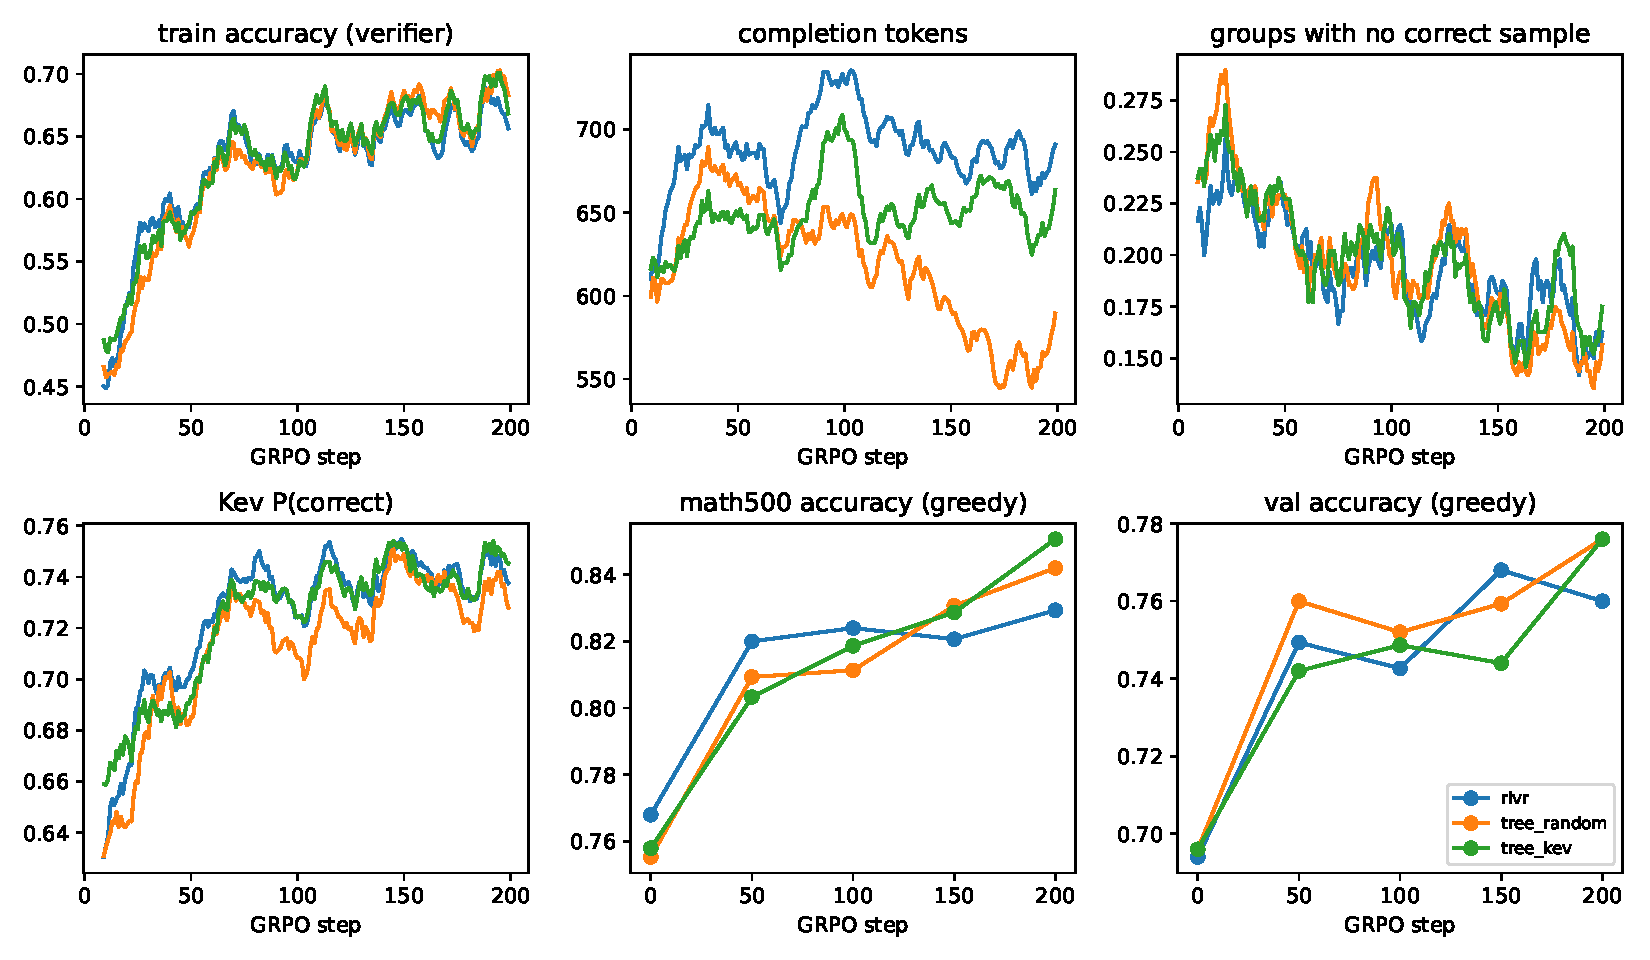
\includegraphics[width=\linewidth]{../../experiments/part3c_tree/results/training_curves.pdf}
\caption{训练曲线（种子均值）：验证器准确率、解答词元数、没有任何正确解答的组的比例，以及 \kev{} 对训练解答给出的 $\pc$（10 步滑动平均）；每 50 步在 MATH-500 和验证集上的贪心准确率。}
\label{fig:tree-curves}
\end{figure}

\paragraph{评估噪声。} 在这一比较的 \NUM{szruns_math500} 个 run 中，基座模型在第 0 步的 MATH-500 准确率介于 \NUM{szmin_math500}\% 和 \NUM{szmax_math500}\% 之间；一个 run 在第 150 步和第 200 步两次评估之间的准确率平均变化 \NUM{lecabs_math500} 个百分点。每个 run 的最终权重都在 MATH-500 上以贪心解码评估了两次：一次是第 200 步的定期评估，一次是最终评估。两次结果平均相差 \NUM{rptabs_math500} 个百分点，最多相差 \NUM{rptmax_math500}（\NUM{rptruns_math500} 个 run）。两次单独评估之间一个百分点左右的差异，在评估本身的噪声之内。
